\chapter{Teorie}
\newacronym{er}{ER}{Entity-Relationship}
\newacronym{uml}{UML}{Unified Modeling Language}
\newacronym{vsk}{VSK}{Vizualizace schematické kategorie}

V~této kapitole představíme potřebné teoretické koncepty, které bude využívat výsledná aplikace.
Mezi tyto koncepty patří \acrfull{er} model a nově vyvíjený konceptuální model v podobě schematické kategorie~\cite{svoboda_categorical_2021} v rozšířené verzi navržené vedoucím práce.

\section{Entity Relationship}\label{section:entity-relationship}

Datový model \acrfull{er} poprvé představil Peter Pin-Shan Chen už v~roce 1976~\cite{chen_er_1976}.
Od té doby se však \acrshort{er} vyvíjel, jak se potřeby datového modelování rozšiřovaly.
\acrshort{er} není standardizováno, ale jednu moderní verzi představili Atzeni, Ceri, Paraboschi a Torlone~\cite[s.~163-179]{atzeni_database_1999}.
Na jejich \acrshort{er} modelu založíme ten náš, který zde popíšeme.

V~Tabulce~\ref{tab:er-constructs} jsou vyobrazeny jednotlivé konstrukty \acrshort{er} modelu.
Zde blíže popíšeme sémantiku jednotlivých konstruktů:
\begin{itemize}
  \item Entitní typ (Entity Type) reprezentuje předpis pro instance entit reálného světa.
        Každý entitní typ má jméno, které je unikátní v daném schématu.
  \item Vztahový typ (Relationship Type) reprezentuje vztah mezi dvěma nebo více (ne nutně různými) entitními typy.
        Každý vztahový typ má jméno.
  \item Atribut (Attribute) reprezentuje vlastnost entitních nebo vztahových typů.
        Každý atribut má jednoznačné jméno.
  \item Složený atribut (Composite Attribute) je atribut, který má sám atributy.
        Zakazujeme však další větvení, tedy atributy složeného atributu už samy nemohou být složené.
        Každý složený atribut má sám jméno, podobně jako jeho vlastní atributy.
  \item \label{def:cardinality}Kardinalita (Cardinality) je dvojice $(a, b) \in \set{\zero, \one}\times \set{\one, \many}$, kde $a$ nazýváme minimální kardinalita (spodní hranice) a $b$ maximální kardinalita (horní hranice).
        Kardinalitu musí mít všechny atributy a každý účastník vztahového typu.
        Výchozí kardinalita je $(1, 1)$ a ve schématu se většinou neuvádí.
        Spodní hranice 0 znamená, že účast je volitelná; hranice 1 znamená, že účast je povinná.
        Horní hranice 1 znamená, že účast je nejvýše jedna; hranice~\many{} znamená, že účastí je libovolný počet.
        \begin{itemize}
          \item Hranice kardinalit pro jednotlivé účastníky vztahů vyjadřují minimální a resp. maximální počet výskytů jednotlivých instancí účastníků v~tomto vztahu.
          \item Hranice kardinalit u~atributů vyjadřují minimální a resp. maximální počet hodnot atributu, které se vztahují k dané instanci entity/vztahu.
        \end{itemize}
  \item Identifikátor (Identifier) umožňuje jednoznačně rozlišit (identifikovat) instance entitních typů.
        Pro každý entitní typ je povinný alespoň jeden identifikátor, ale může jich být více.
        Každý identifikátor je tvořen buď
        \begin{itemize}
          \item jedním nebo více atributy daného entitního typu; takový identifikátor nazýváme interní, nebo
          \item jedním, nebo více vztahovými typy, jichž se daný entitní typ účastní, případně kombinací s~předchozím; takový identifikátor nazýváme externí.
        \end{itemize}
  \item Zobecnění (generalization), nebo také ISA hierarchie\footnote{ISA z anglického \enquote{is a}, analogicky ke vztahu \enquote{has a}} (ISA hierarchy), vyjadřuje vztah podobný dědičnosti v objektově orientovaném programování.
        Jde o vztah mezi entiním typem $E$ zvaným \emph{rodič} a jedním nebo více \emph{dětmi} $E_1, \dots, E_n$.
        Všechny vlastnosti rodiče (atributy, identifikátory, spojené vztahové typy a další ISA hierarchie) jsou i vlastnosti každého z dětí.
        Každá instance dítěte je také instancí rodiče.
\end{itemize}

Entitní typy, které nemají ani jeden interní identifikátor (musí mít tedy externí), nazýváme \emph{slabé} entitní typy (weak entity types).
Pokud mají interní identifikátor, nazýváme je \emph{silné} entitní typy (strong entity types).

Jednoho vztahového typu se může účastnit nejvýše jeden slabý entitní typ, protože pro dva takové by byla identifikace nesmyslná.
Externí identifikace se však může řetězit, jako na Obrázku~\ref{fig:er-external-identifier-chain}.
Nesmí ovšem vzniknout orientovaný cyklus, a to ani v kombinaci s ISA hierarchiemi.
Formálněji -- pokud vytvoříme orientovaný graf $G=(V,E)$ takový, že
\begin{itemize}
  \item vrcholy $V$ jsou entitní typy a
  \item hrany $E$ se skládají z
        \begin{itemize}
          \item pro externí identifikátory orientované hrany od identifikovaného k identifikujícímu entitnímu typu,
          \item pro ISA hierarchii pro každý vztah rodič-dítě, kde $a$ je dítě a $b$ je rodič, orientovanou hranu $(a, b)$,
        \end{itemize}
\end{itemize}
pak graf $G$ musí být acyklický.

Entitní typ, který má externí identifikátor, musí být účastněn vztahového typu (jímž je identifikován) s kardinalitou $(\one,\one)$.
To proto, že když je instance entity identifikována vztahovým typem, musí tento vztah být jednoznačný -- právě jeden.

\begin{figure}[!htb]
  \centering
  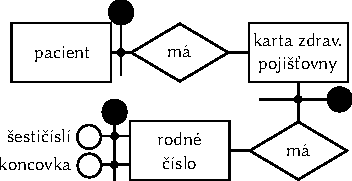
\includegraphics[width=\maxwidth{\textwidth}]{../img/er-model/external-id-chain.pdf}
  \caption{Zřetězení externích identifikátorů}
  \label{fig:er-external-identifier-chain}
\end{figure}

U~kardinality poznamenejme, že se v~\acrshort{er} modelu často dovoluje použít jako hranice libovolná nezáporná celá čísla, tedy $(a, b)\in \mathbb N_0\times \left(\mathbb N_0 \cup \set{\many}\right)$, tž.~$a\leq b$ (dodefinujeme $\forall a\in\mathbb N_0\colon a < \many$).
Dají se tak vyjádřit přesnější omezení, např. že jeden uživatel může mít maximálně 5 bankovních účtů.
Ovšem námi definované hranice kardinality vyjadřují volitelnost/povinnost pro spodní hranici a jednočetnost/mnohočetnost pro horní hranici.
Pokryjeme jimi z teoretického pohledu a s ohledem na povahu konstruktů v nejrůznějších logických modelech všechny strukturálně odlišné situace, které by mohly nastat.

Dále upozorněme, že místo~\many{} se v~\acrshort{er} modelu může použít symbol \texttt{n} nebo \texttt{N} pro vyjádření \enquote{libovolného počtu}.
Důležitá je ale konzistentnost, aby se v~jednom modelu nevyskytovaly dva různé symboly, což by mohlo zmást čtenáře.
V~této práci budeme používat pouze symbol~\many{}.

\begin{table}[!htb]
  \centering
  \begin{tabular}{@{}rm{9cm}@{}} \toprule
    Konstrukt             & Vizuální reprezentace                                     \\ \midrule
    Entitní typ           & {\centering
\includegraphics{../img/er-model/entity.pdf}}  \\
    Vztahový typ          & 
\includegraphics{../img/er-model/relationship.pdf}        \\
    Atribut               & 
\includegraphics{../img/er-model/attribute.pdf}           \\
    Složený atribut       & 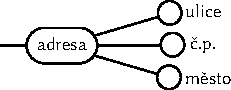
\includegraphics{../img/er-model/composite-attribute.pdf} \\
    Interní identifikátor & 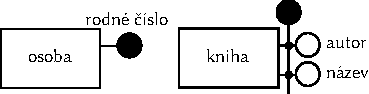
\includegraphics{../img/er-model/identifier.pdf}          \\
    Externí identifikátor & 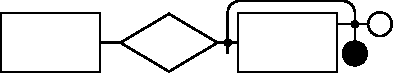
\includegraphics{../img/er-model/external-identifier.pdf} \\
    Zobecnění             & 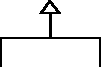
\includegraphics{../img/er-model/generalization.pdf}      \\ \bottomrule
  \end{tabular}
  \caption[Grafická reprezentace konstruktů \acrshort{er} modelu]{Grafická reprezentace konstruktů \acrshort{er} modelu, upraveno a přeloženo~\cite[s.~164, Obr.~5.4]{atzeni_database_1999}}
  \label{tab:er-constructs}
\end{table}

\section{Schematická kategorie}\label{section:schemcat}

V této sekci popíšeme mechanismus pro konceptuální modelování s názvem schematická kategorie společně s teorií kategorií, na které je založena.
Nejdříve ale představíme motivaci za uvedením nového způsobu konceptuálního modelování.

\subsection{Motivace}\mcomment{Tady se musím více rozepsat}

Při začátku vývoje databázových systémů bylo popsáno několik databázových modelů dat.
Už v roce 1975 je ANSI rozdělila do tří vrstev~\cite{steeljr._interimreport_1975}.
\begin{itemize}
  \item Konceptuální vrstva popisuje část světa, na kterou vymezujeme svůj diskurz.
  \item Logická vrstva popisuje logickou strukturu dat (např. graf, tabulka, \dots).
  \item Fyzická vrstva popisuje, jak jsou data fyzicky uložena v paměťové jednotce.
\end{itemize}

Přestože databázových modelů bylo navrženo několik, časem se ukázalo, že nejužitečnější je ten relační.
To proto, že data byla často tabulkové povahy.
Pokud výjimečně nebyla takové povahy, musela se relačnímu modelu přizpůsobit.

S příchodem potřeby zpracování velkých dat (big data) se ukázalo, že relační model není dostačující.
Ve velkém množství dat, která spolu nutně nesouvisí, není totiž jednoduché najít tabulkovou strukturu.
V různých situacích jsou tedy vhodné různé databázové systémy.
Dokonce se začalo používat více databázových systémů najednou.
Například pro cache lze použít key/value store, pro data různorodé povahy lze použít dokumentové databáze a pro strukturovaná data starší relační databáze.

Vize do budoucna je mít jediný databázový systém, který má jediné rozhraní, jediný způsob modelování dat a jediný dotazovací jazyk, ale zároveň není závislý na fyzické vrstvě.
V současných systémech je často tvorba a iterace databázových schémat časově náročná a obtěžující.
Chceme proto sloučit konceptuální a logickou vrstvu a předejít tak problémům a lidskému rozhodování při převodu mezi nimi.
Vznikne tak pouze jedna vrstva, ve které se pracuje unifikovaným, konceptuálním způsobem.

Prvním krokem v této vizi jsou schematické kategorie, které uživateli umožní popsat strukturu dat, se kterými chce v databázi pracovat.
Jejich koncept popisují Martin Svoboda, Pavel Čontoš a Irena Holubová~\cite{svoboda_categorical_2021}.

Prostředky \acrshort{er} jsou vhodné ke konceptuálnímu modelování, nicméně mají několik nevýhod.
Některé z nich zde identifikujeme.
\begin{itemize}
  \item V~\acrshort{er} lze modelovat jeden případ mnoha způsoby a není předem jasné, který z nich je nejlepší.
        Schematické kategorie většinu takových rozdílů smažou, zejména rozdíly mezi entitními typy, vztahovými typy a atributy.
        Často totiž tyto rozdíly nejsou důležité.
  \item \acrshort{er} zavádí několik omezení, např.~vztahové typy nemohou mít interní identifikátor a složené atributy se nemohou libovolně větvit.
        Tato omezení vznikají, protože se historicky \acrshort{er} používalo zejména pro konceptuální modelování pro relační databáze.
        Libovolně větvené atributy se těžko převedou do relačního modelu.
        \acrshort{er} tedy zavádí omezení kvůli logické vrstvě.
        Vyjadřovací síla schematických kategorií je větší, mj. protože není omezena na model logické vrstvy.
\end{itemize}

\acrfull{uml}~\cite{omg_uml_2017} také umožňuje vytvářet konceptuální schémata.
Při vývoji software, zvlášť při práci v týmech, je většinou zvoleno \acrshort{uml} oproti \acrshort{er}.
Je to dáno existencí rozličných nástrojů na kresbu \acrshort{uml} diagramů a nástrojů na automatizaci převodu do logické vrstvy.
Vyjadřovací schopnost \acrshort{uml} je nicméně menší, než u \acrshort{er}.
Postupným vývojem \acrshort{uml} se expresivnost dodává.
Nicméně dosahuje se toho přes konstrukty (např.~stereotypy), u kterých lze poznat, že nesouhlasí s původní myšlenkou \acrshort{uml}.

\subsection{Teorie kategorií}

Nejdříve popíšeme kategorii z~teorie kategorií, na níž je schematická kategorie založena.

Kategorie je matematická struktura, která zobecňuje mnoho jiných matematických struktur.
Umožňuje tak mimo jiné studovat vztahy mezi nimi.
Poprvé byla představena Eilenbergem a MacLanem v~roce 1945~\cite{eilenberg_generaltheory_1945}.

Kategorie $C=(\mathcal O, \mathcal M, \circ)$ se skládá
z~\begin{itemize}
  \item množiny objektů $\mathcal O$,
  \item množniy morfismů $\mathcal M$; každý morfismus $f \in \mathcal M$ má zdrojový objekt $A\in\mathcal O$, cílový objekt $B\in\mathcal O$ a zapisujeme $f: A\to B$ ($f$ je morfismus z~$A$ do $B$),
  \item operace skládání $\circ\colon \mathcal M\times\mathcal M \to \mathcal M$; pro každé dva morfismy $f,g\in\mathcal M$, tž. $f\colon A\to B, g\colon B\to C$, musí $g\circ f\in \mathcal M$ (tranzitivita); pro tuto operaci navíc platí axiomy:
        \begin{itemize}
          \item asociativita -- pro morfismy $f,g,h\in\mathcal M$ takové, že $f\colon A\to B, g\colon B\to C, h\colon C\to D$, platí $h\circ (g \circ f) = (h\circ g)\circ f$,
          \item identitní morfismy -- pro každý morfismus $f\in\mathcal M, f\colon A\to B$ a jeho objekty $A$, resp. $B\in\mathcal O$ existují morfismy $1_A$, resp. $1_B\in\mathcal M$, tž. $f\circ 1_A = f = 1_B\circ f$; morfismy $1_A$, resp. $1_B$ nazýváme \emph{identitní morfismy}.
        \end{itemize}
\end{itemize}

Objekty a morfismy lze definovat i obecněji s použitím tříd místo množin, ale pro naše účely budou stačit množiny.

Jako jednoduchý příklad kategorie uvedeme reálná čísla s neostrou nerovností $(\R, \leq)$. Objekty této kategorie jsou reálná čísla $\mathcal O=\R$.
Pro každá reálná čísla $A,B\in\R$ a morfismus $f\colon A\to B$ je $f\in\mathcal M\iff A\leq B$.
Pro všechny morfismy $f,g\in\mathcal M$ a objekty $A, B, C\in\mathcal O$ takové, že $f\colon A\to B$ a $g\colon B\to C$ definujme $g\circ f=A\to C$.

\begin{statement*}
  $(R, \leq)$ je kategorie.
\end{statement*}
\begin{proof}
  Ověříme postupně všechny axiomy.
  Vezměme libovolné $f,g\in\mathcal M$ a $A,B,C\in\mathcal O$ takové, že $f\colon A\to B$ a $g\colon B\to C$.
  \begin{description}
    \item[uzavřenost na skládání] Z našich definic pro $f,g$ platí $A\leq B\land B\leq C$.
      Z toho plyne $A\leq C$.
      Protože z definice $g\circ f = A\to C$, platí $g\circ f\in\mathcal M$.
    \item[asociativita] Vezměme libovolný morfismus $h\in\mathcal M$ a objekt $D\in\mathcal O$ takový, že $h\colon C\to D$.
      Ověříme, že $h\circ (g\circ f) = (h\circ g)\circ f$.
      \begin{align*}
        h\circ (A\to C) & = (B\to D) \circ f \\
        A\to D          & = A\to D           \\
      \end{align*}
    \item[identitní morfismy] Nechť $1_A =A\to A$ a $1_B = B\to B$.
      Protože platí $A\leq A\land B\leq B$, pak $1_A\in \mathcal M\land 1_B\in\mathcal M$ z definice našich morfismů.
      Nyní ověříme, že $1_A$ a $1_B$ splňují náš požadavek.
      \begin{gather*}
        f\circ 1_A = f = 1_B\circ f \\
        (A\to B)\circ (A\to A) = (A\to B) = (B\to B)\circ (A\to B) \\
        A\to B = A\to B = A\to B \\
      \end{gather*}
  \end{description}
\end{proof}

Kategorie je možné vizuálně reprezentovat orientovaným multigrafem, kde vrcholy jsou objekty a hrany morfismy.
Příklad této vizualizace je na Obrázku~\ref{fig:category-example}.
Jedná se o kategorii se třemi objekty $A, B, C$.
Všimněme si, že každý objekt má svůj identitní morfismus.

\begin{figure}[!htb]
  \shorthandoff{"}
  \centering
  % https://tikzcd.yichuanshen.de/#N4Igdg9gJgpgziAXAbVABwnAlgFyxMJZABgBpiBdUkANwEMAbAVxiRAEEQBfU9TXfIRQBGclVqMWbAELdeIDNjwEio4ePrNWiEAGFu4mFADm8IqABmAJwgBbJGRA4ISURK1sLcyzfuI3zkgATNSaUjrG3iDWdg7UgYgh7uEgxgA6aQDGWFaZAARe1Ax0AEYwDAAK-MpCIFZYxgAWOFExfo4JjgwQEGhEQQDsZBaMcDDixWWV1YJs9U0toZLaIMIA+pw8PrH+8S67IN29RACcw6PjRaXlVUqzOvPNIEseOuuyW9G+wXs-hz19FBnUgjBhjCbXaZ3FQPBpPF4pdb6LgULhAA
  \begin{tikzcd}
    A \arrow[r, "f"] \arrow[rd, "g\circ f"'] \arrow["1_A"', loop, distance=2em, in=215, out=145] & B \arrow[d, "g"] \arrow["1_B"', loop, distance=2em, in=35, out=325] \\
    & C \arrow["1_C"', loop, distance=2em, in=35, out=325]
  \end{tikzcd}
  \caption{Příklad kategorie}%
  \label{fig:category-example}%
  \shorthandon{"}
\end{figure}

\subsection{Schematická kategorie}

Schematická kategorie je mechanismus na popis konceptuálního schématu dat založený na teorii kategorií.
Oproti~\acrshort{er} má schematická kategorie větší vyjadřovací sílu.
Její koncept společně s algoritmem převodu z~\acrshort{er} schématu do schematické kategorie uvádí Martin Svoboda, Pavel Čontoš a Irena Holubová~\cite{svoboda_categorical_2021}.
My však použijeme upravenou definici schematické kategorie navrženou vedoucím práce.

\begin{definition}[Signatura]\label{def:signature}
  Signatura je řetězec nad libovolnou abecedou symbolů $\Sigma$.
  Pokud je signatura řetězec složený z jediného symbolu, říkáme jí \emph{identita}.
  Prázdný řetězec značíme $\varepsilon$.
  Operaci zřetězení značíme symbolem $\cdot$ tečky.
\end{definition}

\begin{example}[Signatury nad $\N$]
  $\varepsilon$, $13$, $13\cdot 7$.
\end{example}

Formálně je schematická kategorie instance kategorie $(\mathcal O, \mathcal M, \circ)$ taková, že
\begin{itemize}
  \item každý objekt této kategorie má strukturu trojice: (identita, název, množina identifikátorů), kde
        \begin{itemize}
          \item identita je libovolný symbol (např.~z~$\N$), který rozlišuje a unikátně identifikuje všechny objekty, které mají ostatní složky totožné (tedy speciálně i pro případ, kdy by všechny ostatní složky byly totožné),
          \item název reprezentuje textovým řetězcem uživatelské jméno daného objektu,
          \item množina identifikátorů obsahuje identifikátory; každý identifikátor je množina identit a vyjadřuje, čím lze daný objekt konceptuálně identifikovat (podobně jako identifikátory z~\acrshort{er}),
        \end{itemize}
  \item každý morfismus má strukturu osmice: (signatura, doména, kodoména, směr, název, kardinalita, duplicity, uspořádání),
        \begin{itemize}
          \item signatura je řetězec z Definice~\ref{def:signature}; buď unikátně identifikuje morfismus v daném schématu (pak je to identita), nebo se jedná o řetězec vyjadřující orientovanou cestu, složený ze signatur jiných morfismů (zřetězujeme ve stejném pořadí jako se zapisuje skládání morfismů v kategorii, viz Obrázek~\ref{fig:morphism-signatures}),
          \item doména a kodoména odpovídají zdrojovému a cílovému objektu tohoto morfismu,
          \item směr je buď \zero{} (tam) nebo \one{} (zpět) s výchozí hodnotou \zero{}; hodnota \one{} vyjadřuje, že tento morfismus je pouze inverze k jinému, dodaná pro úplnost modelu,
          \item název je uživatelské jméno tohoto morfismu, může být i prázdné $\bot$,
          \item kardinalita je dvojice (min, max), která odpovídá kardinalitě z~\acrshort{er} v Sekci~\ref{def:cardinality},
          \item duplicity a uspořádání jsou booleovské hodnoty (\texttt{true}/\texttt{false}), které konceptuálně modelují, zda jsou pro vztažené instance (modelovány kodoménou), která jsou vztažena k vztahované instanci (modelována doménou), povoleny duplicity, resp. jestli mají být uspořádány; tyto hodnoty mají význam pouze pokud je horní hranice kardinality tohto morfismu \many; výchozí hodnota obou složek je \texttt{false}.
        \end{itemize}
\end{itemize}

Morfismy schematické kategorie rozdělíme na několik vzájemně disjunktních druhů.
Příklad každého druhu lze pozorovat na Obrázku~\ref{fig:morphism-signatures}.
\begin{itemize}
  \item \emph{Bázové} (base) morfismy jsou ty, které vyjadřují konceptuální spojení dvou objektů ze schématu (tedy odpovídají jednotlivým spojením z ER); jejich signatura je identita (unikátní symbol z abecedy).
  \item \emph{Identitní} (identity) morfismy jsou ty, které vznikly jen kvůli splnění stejnojmenného axiomu z definice kategorie; jejich signatura je $\varepsilon$.
  \item \emph{Odvozené} (derived) morfismy jsou ty, které vznikly kvůli tranzitivitě (tedy aby byly morfismy uzavřené na operaci skládání); jejich signatura je opravdová cesta -- zřetězené signatury morfismů, ze kterých byl tento morfismus vytvořen.
\end{itemize}

Operaci skládání morfismů $\circ$ ve schematické kategorii lze definovat následovně.
Pro dva morfismy $f,g\in\mathcal M$ a objekty $A,B,C\in \mathcal O$ takové, že $f\colon A\to B, g\colon B\to C$ a
\begin{itemize}
  \item $f$ se skládá z $(\sig_1, \dom_1, \cod_1, \dir_1, \name_1, (\minn_1, \maxx_1), \dup_1, \ord_1)$,
  \item $g$ se skládá z $(\sig_2, \cod_1, \cod_2, \dir_2, \name_2, (\minn_2, \maxx_2), \dup_2, \ord_2)$,
\end{itemize}
je jejich složením $g\circ f$ morfismus $h\in M, h\colon A\to C$ skládající se z
\begin{multline*}
  (\sig_2\cdot \sig_1, \dom_1, \cod_2, \dir_1, \bot, (\min(\minn_1, \minn_2), \max(\maxx_1, \maxx_2)),\\ 
  \dup_1 \lor \dup_2, \ord_1\lor \ord_2)\,.
\end{multline*}

Protože $f$ a $g$ na sebe navazují, musí platit $dir_1=dir_2$, směr morfismů je stejný a směr složeného morfismu bude také stejný.
Dále, protože $dom_1, cod_1, dom_2$ a $cod_2$ odpovídají identitám objektů objektů $A, B, C,$ resp. $D$, složený morfismus má doménu $dom_1$ a kodoménu $cod_2$.
Když u jednoho z morfismů záleží na duplicitách, resp. uspořádání, \hlcomment{bude záležet u složeného morfismu také na duplicitách, resp. uspořádání}{je to pravda?}.

\begin{figure}[!htb]
  \centering
  \begin{tikzpicture}
    \tikzset{vertex/.style={shape=circle,draw,minimum size=1em}}
    \tikzset{edge/.style = {->,> = latex'}}
    \node[vertex] (a) {};
    \node[vertex] (b) [right=of a] {};
    \node[vertex] (c) [right=of b] {};

    \draw[edge] (a) to[bend left] node[above] {$13$} (b) ;
    \draw[edge] (b) to[bend left] node[above] {$7$}  (c);
    \draw[edge] (a) to[bend right] node[below] {$7\cdot 13$} (c);
    \draw[edge] (a) to[loop left] node[left] {$\varepsilon$} (a);
    \draw[edge] (b) to[loop above] node[above] {$\varepsilon$} (b);
    \draw[edge] (c) to[loop right] node[right] {$\varepsilon$} (c);
  \end{tikzpicture}
  \caption{Signatury morfismů, $\cdot$ je operace konkatenace (zřetězování) symbolů}
  \label{fig:morphism-signatures}
\end{figure}

Na Obrázku~\ref{fig:raw-schemcat} je příklad schematické kategorie se třemi objekty.
Objekt \enquote{osoba} je identifikován dohromady dvojicí objektů \enquote{jméno} a \enquote{příjmení}.
Objekty \enquote{jméno} a \enquote{příjmení} jsou každý identifikován sám sebou, proto jim náleží identifikátor $\set{\varepsilon}$.
Na obrázku jsou dále bázové morfismy (černé čáry) se svými identitami a kardinalitami.
Odvozené a identitní morfismy jsou vyznačeny šedivými křivkami.
Jejich signatury jsou složené řetězce, resp. prázdné řetězce $\varepsilon$.

\begin{figure}[!htb]
  \centering
  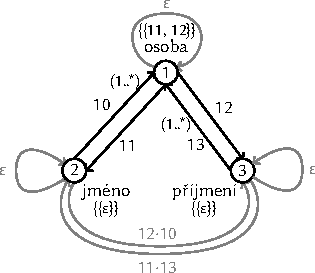
\includegraphics[width=\maxwidth{\textwidth}]{../img/schemcat-diagrams/raw-schemcat-example.pdf}
  \caption[Příklad schematické kategorie]{Příklad schematické kategorie. Identifikátory jsou vyobrazeny množinovým zápisem. Výchozí kardinalita je (\one, \one) a neuvádí se.}
  \label{fig:raw-schemcat}
\end{figure}

\section{Vizualizace schematické kategorie}\label{section:vsk}

Schematická kategorie je formální, pečlivě zadefinovaný model.
Pro potenciálního uživatele schematické kategorie je její jednolitost a informativnost příliš nepřehledná.
Navrhněme proto způsob vizualizace, který přinese odlišení a zvýraznění některých důležitých konstruktů, včetně vyobrazení některých složek objektů a morfismů.
Pojmenujme ho \acrfull{vsk}.

Objekt schematické kategorie, který má v identifikátorech $\set{\varepsilon}$ nazveme \emph{self-identifikovaný} objekt.
Instance takových objektů jsou identifikovány svými hodnotami.
Jsou tedy podobné atributům z \acrshort{er} a proto je budeme značit podobným tvarem.

Objekty, které nejsou self-identifikované, jsou určitě identifikované jinými objekty.
Jsou významově podobné entitním typům z \acrshort{er}, a proto je budeme značit stejným tvarem.

Ve \acrshort{vsk} nebudou viditelné identity objektů.

Morfismy budeme značit spojovacími čárami mezi objekty.
Inverzní morfismy (ty, které mají směr \enquote{zpět}) vyobrazovat nebudeme.
Nebudeme vizualizovat ani identitní a odvozené morfismy.
Neukážeme ani signatury zbývajících morfismů.

Kardinality morfismů budeme vykreslovat u patřičného morfismu stejným zápisem, jako u \acrshort{er}.
Pokud je však kardinalita výchozí (\one, \one), budeme ji považovat za implicitní a nezobrazíme ji.
Pokud má morfismus $A$ inverzní morfismus $A^{-1}$ (ten nezobrazíme), pak
\begin{itemize}
  \item kardinalitu morfismu $A$ budeme značit blízko cílového objektu $A$
  \item a kardinalitu morfismu $A^{-1}$ budeme značit blízko zdrojového objektu $A$.
\end{itemize}

Identifikátory objektů budeme značit stejně jako v \acrshort{er} přeškrtnutím patřičných morfismů.

Složky morfismu \emph{uspořádání} a \emph{duplicity} budou pro výchozí hodnoty (\texttt{false} a \texttt{false}) neviditelné.
Jinak v cílovém objektu na konci spojovací čáry morfismu vyznačíme pravdivou hodnotu uspořádání symbolem $<$, resp. $+$ pro duplicity.

Uživatelské názvy objektů i morfismů budeme vykreslovat, podobně jako v \acrshort{er}, u self-identifikovaných objektů v blízkosti objektu, jinak uvnitř obdélníku ne-self-identifikovaného objektu.

Na Obrázku~\ref{fig:schemcat-visualization-example} vidíme \acrshort{vsk} odpovídající schematické kategorii z Obrázku~\ref{fig:raw-schemcat}.
Sémantika kardinalit (\one, \many) u obou obrázků taková, že konceptuálně může jedno jméno, resp. příjmení patřit více osobám.

Na Obrázku~\ref{fig:scv-ord-dup} lze vidět \acrshort{vsk} schematické kategorie, která má u jednoho z morfismů pravdivé uspořádání a duplicity.
Význam tohoto konceptuálního modelu je takový, že jeden seznam úkolů může mít více úkolů se stejným popisem (duplicity) a že je důležité udržovat informaci o pořadí, ve kterém byly jednotlivé úkoly přidávány (uspořádání).

\begin{figure}[!htb]
  \centering
  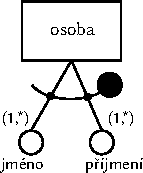
\includegraphics[width=\maxwidth{\textwidth}]{../img/schemcat-diagrams/schemcat-visualization-example.pdf}
  \caption{Příklad \acrfull{vsk}.}
  \label{fig:schemcat-visualization-example}
\end{figure}

\begin{figure}[!htb]
  \centering
  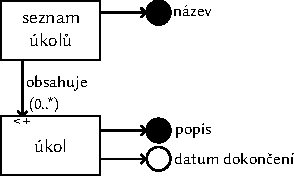
\includegraphics[width=\maxwidth{\textwidth}]{../img/schemcat-diagrams/scv-ord-dup.pdf}
  \caption{\acrshort{vsk} pro schematickou kategorii s využitými složkami \emph{uspořádání} a \emph{duplicity}.}
  \label{fig:scv-ord-dup}
\end{figure}

Všimněme si, že žádná informace schmetické kategorie se ve \acrshort{vsk} neztratí.
Pokud nějaká informace není zobrazena, znamená to, že má definovanou výchozí hodnotu.
Díky tomu lze říci, že \acrshort{vsk} a schematická kategorie jsou na sebe vzájemně převoditelné a tedy jsou ekvivalentní.

\section{Převod ER na schematickou kategorii}

Algoritmus převodu z~\acrshort{er} na schematickou kategorii už popsali Svoboda a kol.~\cite[s.~192-196]{svoboda_categorical_2021}.
Pro naši upravenou verzi schematické kategorie musíme upravit i algoritmus převodu.

Mějme tedy validní \acrshort{er} diagram.
Převedeme ho na schematickou kategorii.
Představme k tomu Algoritmus~\ref{alg:conversion-er-schemcat}.

\begin{algorithm}[htb]
  \DontPrintSemicolon
  \SetKwFor{For}{pro}{dělej}{konec}
  \SetKwFor{While}{dokud}{dělej}{konec}
  \SetKwFor{ForAll}{pro\ každý}{dělej}{konec}
  \SetKwProg{Fn}{funkce}{ je}{konec}
  \SetKw{Return}{vrať}%
  $\mathcal S\gets$ prázdná schematická kategorie\;
  $\Sigma \gets $ libovolná abeceda, např.~$\N$\;
  \Fn{vytvořObjekt(název)}{
    $i\gets$ unikátní symbol z $\Sigma$\;
    \tcp{(identita, název, množina identifikátorů)}
    $O\gets$ (i, název, $\set{}$)\;
    vlož $O$ do objektů $\mathcal S$\;
    \Return $O$\;
  }
  \Fn{vytvořBázovýMorfismus(dom, kod, název, kardinalitaTam, kardinalitaZpět)}{
    $i\gets$ unikátní symbol z $\Sigma$\;
    $j\gets$ unikátní symbol z $\Sigma$\;
    \tcp{(signatura, doména, kodoména, směr, název, kardinalita, duplicity, uspořádání)}
    $M\gets$ (i, dom, kod, 0, název, kardinalitaTam, \texttt{false}, \texttt{false})\;
    $M^{-1}\gets$ (j, dom, kod, 1, název, kardinalitaZpět, \texttt{false}, \texttt{false})\;
    vlož $M$ a $M^{-1}$ do morfismů $\mathcal S$\;
    \Return $M$\;
  }
  označ všechny entitní typy z $\mathcal S$ za \emph{nevyřešené}\;
  \ForAll{nesložený atribut $A$ z \acrshort{er} diagramu}{
    $O_A\gets$ vytvořObjekt(jméno $A$)\;
    do množiny identifikátorů $O_A$ vlož $\set{\varepsilon}$\;
  }
  \For{složený atribut $C$ z \acrshort{er} diagramu}{
    $O_C\gets$ vytvořObjekt(jméno $C$)\;
    \For{atribut $A$, který náleží $C$}{
      $O_A\gets$ objekt z $\mathcal S$ odpovídající atributu $A$\;
      $M_A\gets$ vytvořBázovýMorfismus(identita $O_C$, identita $O_A$, $\bot$, (\one{}..\one{}), (\one{}..\many{}))\;
    }
    do množiny identifikátorů $O_C$ přidej množinu signatur právě výše vytvořených $M_A$\;
  }
  \caption{Algoritmus převodu \acrshort{er} na schematickou kategorii}
  \label{alg:conversion-er-schemcat}
\end{algorithm}
\begin{algorithm}[htb]
  \DontPrintSemicolon
  \setcounter{AlgoLine}{29}
  \SetKwFor{For}{pro}{dělej}{konec}
  \SetKwFor{While}{dokud}{dělej}{konec}
  \SetKwFor{ForAll}{pro\ každý}{dělej}{konec}
  \SetKwProg{Fn}{funkce}{ je}{konec}
  \SetKwIF{If}{ElseIf}{Else}{pokud}{pak}{jinak pokud}{jinak}{konec}
  \SetKw{Return}{vrať}
  \ForAll{entitní typ $E$ z \acrshort{er} diagramu}{
    %todo dodělat entitní typy, hierarchie, vztahové typy, slabé identifikátory
    $O_E\gets$ vytvořObjekt(jméno $E$)\;
    \ForAll{atribut $A$ entitního typu $E$}{
      $O_A\gets$ objekt z $\mathcal S$ odpovídající atributu $A$
      $M_A\gets$ vytvořBázovýMorfismus(identita $O_E$, identita $O_A$, $\bot$, kardinalita $A$ vzhledem k $E$, (\one..\one))\;
    }
    \ForAll{interní identifikátor $I$ entitního typu $E$}{
      $M_I\gets$ množina morfismů z $\mathcal S$, které vedou k atributům z $I$\;
      přidej do množiny identifikátorů objektu $O_E$ množinu $M_I$\;
    }
    \If{$E$ nemá externí identifikátor}{
      označ $E$ za \emph{vyřešený}\;
    }
  }
  \ForAll{vztahový typ $R$ z \acrshort{er} diagramu}{
    $O_R\gets$ vytvořObjekt(jméno $R$)\;
    \ForAll{atribut $A$ vztahového typu $R$}{
      $O_A\gets$ objekt z $\mathcal S$ odpovídající atributu $A$\;
      $M_A\gets$ vytvořBázovýMorfismus(identita $O_R$, identita $O_A$, $\bot$, kardinalita $A$ vzhledem k $R$, (\one..\one))\;
    }
    \ForAll{entitní typ $E$, který je účastníkem vztahového typu $R$}{
      $O_E\gets$ objekty z $\mathcal S$ odpovídající entitě $E$\;
      $M_E\gets$ vytvořBázovýMorfismus(identita $O_R$, identita $O_E$, $\bot$, kardinalita $E$ vzhledem k $R$, kardinalita $R$ vzhledem k $E$)\;
    }
  }
  \While{existuje nevyřešený entitní typ $E$\label{alg:dokud}}{
    \ForAll{externí identifikátor $I$ entitního typu $E$}{
      $O_E\gets$ objekt z $\mathcal S$ odpovídající entitě $E$\;
      \If{jsou všechny entitní typy $E_V$, do kterých vede externí identifikátor $I$, vyřešené}{
        pro každý $E_i\in E_V$ označ odpovídající $O_i\in\mathcal S$\;
        vytvoř orientovanou cestu přes odpovídající morfismy z $E$ do $E_i$, označ $C_i$\;
        zřetězením vytvoř z každé $C_i$ signaturu $S_i$\;
        \ForAll{identifikátor $I_k$ z množiny identifikátorů $O_i$}{
          $S_f\gets\set{S\cdot S_i\mid S\in I_k}$\;
          přidej $S_f$ do množiny identifikátorů objektu $O_E$\;
        }
        označ $E$ \emph{za vyřešenou}\;
      }
    }
  }
\end{algorithm}
\begin{algorithm}[htb]
  \DontPrintSemicolon
  \setcounter{AlgoLine}{68}
  \SetKwFor{For}{pro}{dělej}{konec}
  \SetKwFor{While}{dokud}{dělej}{konec}
  \SetKwFor{ForAll}{pro\ každý}{dělej}{konec}
  \SetKwProg{Fn}{funkce}{ je}{konec}
  \SetKwIF{If}{ElseIf}{Else}{pokud}{pak}{jinak pokud}{jinak}{konec}
  \SetKw{Return}{vrať}
  \ForAll{vztahový typ $R$ z \acrshort{er} diagramu}{
    $O_R\gets$ objekt z $\mathcal S$ odpovídající $R$\;
    \uIf{se $R$ účastní nějakého externího identifikátoru}{
      do množiny identifikátorů objektu $O_R$ přidej nový identifikátor tvořený odpovídajícími signaturami podobně jako výše\;
    }\uElseIf{alespoň jeden účastník $E$ vztahového typu $R$ je účastněn s kardinalitou, která má horní hranici \one{}}{
      pro každého takového účastníka $E$ vlož do $O_R$ identifikátor odpovídající $E$\;
    }\Else{
      přidej pro každého účastníka $E$ vztahového typu $R$ nový identifikátor do $O_R$ odpovídající $E$\;
    }
  }
  \ForAll{vztah rodič-dítě ($P,C$) z hierarchií \acrshort{er} diagramu}{
    $O_P,O_C\gets$ odpovídající objekty z $\mathcal S$\;
    $M_H\gets$ vytvořBázovýMorfismus(identita $O_C$, identita $O_P$, $\bot$, (\one{}..\one{}), (\one{}..\one{}))\;
    správně dořetězené identifikátory odpovídající všem identifikátorům $O_P$ přidej do identifikátorů $O_C$\;
  }
  do $\mathcal S$ dodej operací skládání morfismů $\circ$ všechny odvozené morfismy chybějící do tranzitivního uzávěru\;
  pro každý objekt $O$ v $\mathcal S$ dodej do $\mathcal S$ identitní morfismus ($\set{\varepsilon}$, identita $O$, identita $O$, \zero{}, $\bot$, (\one{}..\one{}), \texttt{false}, \texttt{false})\;
\end{algorithm}

V algoritmu předpokládáme, že $\Sigma$ má dostatek symbolů, aby šlo po celou dobu běhu algoritmu volit unikátní symbol.

Uvědomme si, že $E$ nemusí mít ani jeden vlastní atribut ze dvou důvodů, které se vzájemně nevylučují:
\begin{enumerate}
  \item $E$ může být dítě v hierarchii, kdy dědí identifikátor od rodiče,
  \item nebo se může jednat o slabý entitní typ, který nemá ani jeden interní identifikátor.
\end{enumerate}

Algoritmus skončí, pokud dostane korektní \acrshort{er} diagram (takže nemá cykly a je konečný), protože v cyklu \emph{dokud} na řádce \ref{alg:dokud} se určitě v každé iteraci najde alespoň jeden řešitelný entitní typ, díky neexistenci cyklů.
